\documentclass[12pt]{article}

% Set the page to be letter paper and have small margins
\usepackage{geometry}
\geometry{letterpaper, left=15mm, right=15mm, top=15mm, bottom=20mm}


% LuaLaTeX font setup
\usepackage{fontspec}
\usepackage{unicode-math}

% Text font
\setmainfont{DejaVu Serif}

% Math font
\setmathfont{STIX Two Math}

\usepackage{parskip}
\usepackage{amsmath}
\usepackage{amsthm}
\usepackage{multicol}
\usepackage{graphicx}
\usepackage{pgfplots}
\pgfplotsset{compat=1.18}
\usepackage{cancel}

\usepackage{enumitem}
% \setlist[enumerate]{font={\bfseries}}
\setlist[enumerate, 1]{label=\textbf{\arabic*}.}
\setlist[enumerate, 2]{label=(\textbf{\alph*})}

% Allow for page breaks between multi-line math environments (gather, align, etc)
\allowdisplaybreaks[1]

\begin{document}

\noindent
Jeffrey Morris
\hfill
MATH 4306-010
\newline
January 26, 2026

\begin{center}
    \Large{Homework 2}
\end{center}

\begin{enumerate}
    \item Given the function $f(x)=x^2$.
          \begin{enumerate}
              \item Find the Fourier series of $f$ over $\left( -\pi,\pi \right)$. \label{1:a}
                    \begin{align*}
                        a_0 & = \frac{1}{2\pi}\int_{-\pi}^{\pi}f(x)\,dx          \\
                        a_0 & = \frac{1}{\pi} \int_{0}^{\pi}x^2\,dx              \\
                        a_0 & = \frac{1}{\pi} \left[ \frac{x^3}{3} \right]_0^\pi \\
                        a_0 & = \frac{\pi^3}{3\pi}                               \\
                        a_0 & =  \frac{\pi^2}{3}
                    \end{align*}
                    \begin{align*}
                        a_n & = \frac{1}{\pi}\int_{-\pi}^{\pi} f(x)\cos(nx)\,dx                                                              \\
                        a_n & = \frac{2}{\pi} \int_{0}^{\pi} x^2\cos(nx)\,dx                                                                 \\
                        a_n & = \frac{2}{\pi} \left[ \frac{x^2}{n} \sin(nx) + \frac{2x}{n^2} \cos(nx) - \frac{2}{n^3} \sin(nx) \right]_0^\pi \\
                        a_n & = \frac{2}{\pi} \left[ \frac{2\pi}{n^2} \cos(n\pi) - 0 \right]                                                 \\
                        a_n & = \frac{2}{\pi} \left[ \frac{2\pi(-1)^n}{n^2} \right]                                                          \\
                        a_n & = \frac{4(-1)^n}{n^2}
                    \end{align*}
                    \begin{center}
                        $
                            \boxed{f(x) = \frac{\pi^2}{3} + \sum_{n=1}^{\infty}\frac{4(-1)^n}{n^2}\cos(nx)}
                        $
                    \end{center}
              \item Using \ref{1:a}, show that $\frac{\pi}{12}=\sum_{n=1}^{\infty} \frac{\left( -1 \right)^{n+1}}{n^2}$.
                    \begin{align*}
                        f(0)              & = \frac{\pi^2}{3} + \sum_{n=1}^{\infty}\frac{4(-1)^n}{n^2}\cos(0) \\
                        \frac{-\pi^2}{3}  & = 4 \sum_{n=1}^{\infty}\frac{(-1)^n}{n^2}                         \\
                        \frac{-\pi^2}{12} & = \sum_{n=1}^{\infty}\frac{(-1)^n}{n^2}                           \\
                        \frac{\pi^2}{12}  & = \sum_{n=1}^{\infty}\frac{(-1)^{n+1}}{n^2}
                    \end{align*}
              \item Using \ref{1:a} and Parseval's identity, show that $\frac{\pi^4}{90}=\sum_{n=1}^{\infty}\frac{1}{n^4}$.
                    \begin{align*}
                        \frac{1}{2L}\int_{-L}^{L}\left| f(x) \right|^2       & = a_0^2 + \frac{1}{2}\sum_{n=1}^{\infty}\left( a_n^2+b_n^2 \right)                                      \\
                        \frac{1}{2\pi} \int_{-\pi}^{\pi}\left| x^2 \right|^2 & = \left( \frac{\pi^2}{3} \right)^2 + \frac{1}{2}\sum_{n=1}^{\infty}\left( \frac{4(-1)^n}{n^2} \right)^2 \\
                        \text{LHS}                                           & = \frac{1}{\pi}\int_{0}^{\pi}x^4\,dx                                                                    \\
                                                                             & = \frac{1}{\pi}\left[ \frac{x^5}{5} \right]_0^\pi                                                       \\
                                                                             & = \frac{\pi^4}{5}                                                                                       \\
                        \text{RHS}                                           & = \left( \frac{\pi^2}{3} \right)^2 + \frac{1}{2}\sum_{n=1}^{\infty}\left( \frac{4(-1)^n}{n^2} \right)^2 \\
                                                                             & = \frac{\pi^4}{9} + \frac{1}{2}\sum_{n=1}^{\infty}\frac{16}{n^4}                                        \\
                                                                             & = \frac{\pi^4}{9} + 8 \sum_{n=1}^{\infty}\frac{1}{n^4}                                                  \\
                        \\
                        \frac{\pi^4}{5}                                      & = \frac{\pi^4}{9} + 8\sum_{n=1}^{\infty} \frac{1}{n^4}                                                  \\
                        \pi^4 \left( \frac{1}{5} - \frac{1}{9} \right)       & = 8\sum_{n=1}^{\infty} \frac{1}{n^4}                                                                    \\
                        \frac{4\pi^4}{45}                                    & = 8\sum_{n=1}^{\infty} \frac{1}{n^4}                                                                    \\
                        \frac{\pi^4}{90}                                     & = \sum_{n=1}^{\infty} \frac{1}{n^4}
                    \end{align*}
          \end{enumerate}
    \item Given the function:
          \begin{center}
              $
                  f(x)=
                  \begin{cases}
                      0,       & \text{if $-\pi < x \leq 0$} \\
                      \sin(x), & \text{if $0 < x \leq \pi$}
                  \end{cases}
              $
          \end{center}
          \begin{enumerate}
              \item Find the Fourier series of $f(x)$ over $\left( -\pi,\pi \right)$. \label{2:a}
                    \begin{align*}
                        a_0 & = \frac{1}{2\pi}\int_{-\pi}^{\pi}f(x)\,dx     \\
                        a_0 & = \frac{1}{2\pi}\int_{0}^{\pi}\sin(x)\,dx     \\
                        a_0 & = \frac{1}{2\pi}\left[ -\cos(x) \right]_0^\pi \\
                        a_0 & = \frac{1}{2\pi}\left[ -(-1) - (-1) \right]   \\
                        a_0 & = \frac{1}{\pi}                               \\
                    \end{align*}
                    \begin{align*}
                        a_n & = \frac{1}{\pi}\int_{-\pi}^{\pi}f(x)\cos(nx)\,dx                                                                                                                                     \\
                        a_n & = \frac{1}{\pi}\int_{0}^{\pi} \sin(x)\cos(nx)\,dx                                                                                                                                    \\
                        a_n & = \frac{1}{\pi}\int_{0}^{\pi} \frac{1}{2} \left[ \sin\left( (n+1)x \right) - \sin\left( (n-1) x \right) \right]\,dx                                                                  \\
                        a_n & = \frac{1}{2\pi} \left[ \frac{-\cos\left( (n+1) x \right)}{n+1} + \frac{\cos \left( (n-1) x \right)}{n-1} \right]_0^\pi                                                              \\
                        a_n & = \frac{1}{2\pi} \left[ \left( \frac{-\cos\left( (n+1) \pi \right)}{n+1} + \frac{\cos \left( (n-1) \pi \right)}{n-1} \right) - \left( \frac{-1}{n+1} + \frac{1}{n-1} \right) \right] \\
                        a_n & = \frac{1}{2\pi} \left[ \frac{(-1)^n}{n+1} + \frac{-(-1)^n}{n-1} + \frac{1}{n+1} + \frac{-1}{n-1} \right]                                                                            \\
                        a_n & = \frac{1}{2\pi} \left[ \frac{1+(-1)^n}{n+1} - \frac{1+(-1)^n}{n-1} \right]                                                                                                          \\
                        a_n & = \frac{1+(-1)^n}{2\pi} \left[ \frac{-2}{n^2-1} \right]                                                                                                                              \\
                        a_n & =
                        \begin{cases}
                            0,                                    & \text{if $n$ is odd}  \\
                            \frac{-2}{\left( n^2 - 1\right) \pi}, & \text{if $n$ is even}
                        \end{cases}
                    \end{align*}
                    \begin{align*}
                        b_n              & = \frac{1}{\pi}\int_{-\pi}^{\pi}f(x)\sin(nx)\,dx                                                                           \\
                        b_n              & = \frac{1}{\pi}\int_{0}^{\pi}\sin(x)\sin(nx)\,dx                                                                           \\
                        b_n              & = \frac{1}{\pi}\int_{0}^{\pi}\frac{1}{2}\left[ \cos\left( (n-1) x \right) - \cos\left( (n+1) x \right) \right]\,dx         \\
                        n=1\qquad b_1    & = \frac{1}{2\pi}\int_{0}^{\pi}1-\cos(2x)\,dx                                                                               \\
                        b_1              & = \frac{1}{2\pi}\left[ x - \frac{\sin(2x)}{2} \right]_0^\pi                                                                \\
                        b_1              & = \frac{1}{2}                                                                                                              \\
                        n\ne1 \qquad b_n & = b_n = \frac{1}{2\pi}\left[ \frac{\sin\left( (n-1) x \right)}{n-1} - \frac{\sin\left( (n+1) x \right)}{n+1} \right]_0^\pi \\
                        b_n              & = 0
                    \end{align*}
                    \begin{align*}
                        f(x) & =\frac{1}{\pi} + \frac{1}{2}\sin(x) + \sum_{\text{$n$ = even}}^{\infty}\frac{-2}{(n^2 -1)\pi}\cos(nx)      \\
                        f(x) & = \boxed{\frac{1}{\pi} + \frac{1}{2}\sin(x) + \frac{-2}{\pi}\sum_{n=1}^{\infty}\frac{\cos(2nx)}{(2n)^2-1}}
                    \end{align*}
              \item Using \ref{2:a} and Parseval's identity, show that:
                    \begin{center}
                        $\frac{\pi^2}{16}-\frac{1}{2}=\sum_{\text{$k =$ even}}^{\infty}\frac{1}{\left( k^2 - 1 \right)^2}.$
                    \end{center}
                    \begin{align*}
                        \frac{1}{2L} \int_{-L}^{L}\left| f(x) \right|^2\,dx & = a_0^2 + \frac{1}{2}\sum_{n=1}^{\infty}a_n^2+b_n^2                                                              \\
                        \text{LHS:}                                         & = \frac{1}{2\pi} \int_{-\pi}^{\pi} \left| f(x) \right|^2                                                         \\
                                                                            & = \frac{1}{2\pi} \int_{0}^{\pi} \sin^2(x)\,dx                                                                    \\
                                                                            & = \frac{1}{2\pi} \int_{0}^{\pi} \frac{1-\cos(2x)}{2}\,dx                                                         \\
                                                                            & = \frac{1}{4\pi} \int_{0}^{\pi} 1 - \cos(2x) \,dx                                                                \\
                                                                            & = \frac{1}{4\pi} \left[ x - \frac{\sin(2x)}{2} \right]_0^\pi                                                     \\
                                                                            & = \frac{1}{4\pi} \left[ \left( \pi - \frac{\sin(2\pi)}{2} \right) - \left( 0 - \frac{\sin(0)}{2} \right) \right] \\
                                                                            & = \frac{1}{4\pi} \cdot \pi                                                                                       \\
                                                                            & = \frac{1}{4}                                                                                                    \\
                        \text{RHS: }                                        & = a_0^2 + \frac{1}{2} \sum_{n=1}^{\infty}a_n^2+b_1^2                                                             \\
                                                                            & = \frac{1}{\pi^2} + \frac{1}{2}\sum_{n=1}^{\infty}\frac{4}{\left( (2n)^2 - 1 \right)^2 \pi^2} + \frac{1}{4}      \\
                                                                            & = \frac{1}{\pi^2} + \frac{1}{8} + \frac{2}{\pi^2}\sum_{n=1}^{\infty}\frac{1}{\left( (2n)^2 - 1 \right)^2}        \\
                        \\
                        \frac{1}{4}                                         & = \frac{1}{\pi^2} + \frac{1}{8} + \frac{2}{\pi^2}\sum_{n=1}^{\infty}\frac{1}{\left( (2n)^2 - 1 \right)^2}        \\
                        \frac{1}{4} - \frac{1}{\pi^2} - \frac{1}{8}         & = \frac{2}{\pi^2} \sum_{n=1}^{\infty} \frac{1}{\left( (2n)^2 - 1 \right)^2}                                      \\
                        \frac{\pi^2 - 8}{8\pi^2}                            & = \frac{2}{\pi^2} \sum_{n=1}^{\infty} \frac{1}{\left( (2n)^2 - 1 \right)^2}                                      \\
                        \frac{\pi^2 - 8}{16}                                & = \sum_{n=1}^{\infty} \frac{1}{\left( (2n)^2 - 1 \right)^2}                                                      \\
                        \frac{\pi^2}{16} - \frac{1}{2}                      & = \sum_{\text{$k$ = even}}^{\infty} \frac{1}{(k^2 - 1)^2}
                    \end{align*}
          \end{enumerate}
    \item Sketch the even and odd extensions of each of the following functions, and find the Fourier cosine and sine integrals for $f$. Each function is given in the interval $0<x<\infty$.
          \begin{enumerate}
              \item $f(x)=e^{-x}$
                    \begin{center}
                        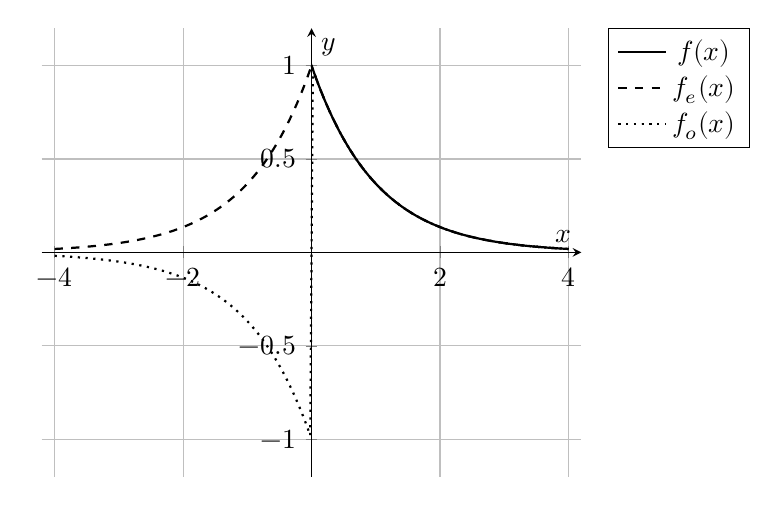
\begin{tikzpicture}
                            \begin{axis}[
                                    axis lines=middle,
                                    grid=both,
                                    xmin=-4.2, xmax=4.2,
                                    ymin=-1.2, ymax=1.2,
                                    samples=200,
                                    xlabel={$x$},
                                    ylabel={$y$},
                                    legend style={at={(1.05,1)},anchor=north west}
                                ]

                                \addplot[thick,domain=0:4] {exp(-x)};
                                \addlegendentry{$f(x)$}

                                \addplot[thick,domain=-4:4,dashed] {exp(-abs(x))};
                                \addlegendentry{$f_e(x)$}

                                \addplot[thick,domain=-4:4,dotted]
                                { (x==0 ? 0 : (x>0 ? exp(-x) : -exp(x))) };
                                \addlegendentry{$f_o(x)$}

                            \end{axis}
                        \end{tikzpicture}
                    \end{center}
                    \begin{align*}
                        f_c(x)          & =\int_{0}^{\infty}A(\lambda)\cos(\lambda x)\,d\lambda                                                                                \\
                        A(\lambda)      & = \frac{2}{\pi} \int_{0}^{\infty} f(x)\cos(\lambda x)\,dx                                                                            \\
                        A(\lambda)      & = \frac{2}{\pi} \int_{0}^{\infty} e^{-x}\cos(\lambda x)\,dx                                                                          \\
                        I               & = \int_{0}^{\infty} e^{-x}\cos(\lambda x)\,dx                                                                                        \\
                        I               & = \left. -e^{-x}\cos(\lambda x)  \right|_0^\infty - \int_{0}^{\infty} e^{-x}\lambda \sin(\lambda x)\,dx                              \\
                        I               & = 1 - \lambda \int_{0}^{\infty} e^{-x}\sin(\lambda x)\,dx                                                                            \\
                        I               & = 1 - \lambda \left[ \left. -e^{-x}\sin(\lambda x)\right|_0^\infty - \int_{0}^{\infty} -e^{-x}\lambda \cos(\lambda x)\,dx \right]    \\
                        I               & = 1 + \cancelto{0}{\left. \lambda e^{-x} \sin(\lambda x) \right|_0^\infty } - \lambda^2 \int_{0}^{\infty} e^{-x} \cos(\lambda x)\,dx \\
                        I               & = 1 - \lambda^2 I                                                                                                                    \\
                        I + \lambda^2 I & = 1                                                                                                                                  \\
                        I               & = \frac{1}{1 + \lambda^2}                                                                                                            \\
                        f_c(x)          & = \int_{0}^{\infty}\frac{2}{\pi}\left[ \frac{1}{1 + \lambda^2} \right] \cos(\lambda x)\,d\lambda                                     \\
                        f_c(x)          & = \boxed{\frac{2}{\pi}\int_{0}^{\infty}\frac{\cos(\lambda x)}{1 + \lambda^2}\,d\lambda}
                    \end{align*}
                    \begin{align*}
                        f_s(x)          & = \int_{0}^{\infty}B(\lambda)\sin(\lambda x)\,d\lambda                                                                         \\
                        B(\lambda)      & = \frac{2}{\pi} \int_{0}^{\infty} f(x)\sin(\lambda x)\,dx                                                                      \\
                        B(\lambda)      & = \frac{2}{\pi} \int_{0}^{\infty} e^{-x} \sin(\lambda x)\,dx                                                                   \\
                        I               & = \int_{0}^{\infty} e^{-x} \sin(\lambda x)\,dx                                                                                 \\
                        I               & = \left. -e^{-x}\sin(\lambda x)\right|_0^\infty - \int_{0}^{\infty} e^{-x} \lambda \cos(\lambda x) \, dx                       \\
                        I               & = \cancelto{0}{\left. -e^{-x}\sin(\lambda x)\right|_0^\infty} - \lambda \int_{0}^{\infty} e^{-x} \cos(\lambda x) \, dx         \\
                        I               & = \lambda \left[ \left. -e^{-x} \cos(\lambda x) \right|_0^\infty - \int_{0}^{\infty} e^{-x}\lambda \sin(\lambda x)\,dx \right] \\
                        I               & = \lambda \left[ -1 - \lambda \int_{0}^{\infty} e^{-x}\sin(\lambda x)\, dx \right]                                             \\
                        I               & = -\lambda - \lambda^2 I                                                                                                       \\
                        I + \lambda^2 I & = -\lambda                                                                                                                     \\
                        I               & = \frac{-\lambda}{1 + \lambda^2}                                                                                               \\
                        f_s(x)          & = \int_{0}^{\infty} \frac{2}{\pi} \left[ \frac{-\lambda}{1 + \lambda^2} \right]\sin(\lambda x)\,d\lambda                       \\
                        f_s(x)          & = \boxed{\frac{2}{\pi} \int_{0}^{\infty} \frac{-\lambda \sin(\lambda x)}{1 + \lambda^2}\,d\lambda}
                    \end{align*}
              \item $
                        f(x)=
                        \begin{cases}
                            1, & 0<x<1 \\
                            0, & 1<x
                        \end{cases}
                    $
                    \begin{center}
                        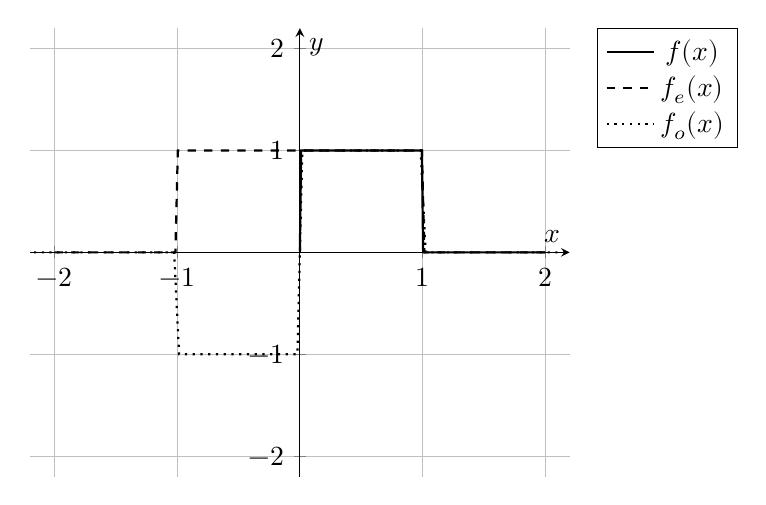
\begin{tikzpicture}
                            \begin{axis}[
                                    axis lines=middle,
                                    grid=both,
                                    xmin=-2.2, xmax=2.2,
                                    ymin=-2.2, ymax=2.2,
                                    samples=200,
                                    xlabel={$x$},
                                    ylabel={$y$},
                                    legend style={at={(1.05,1)},anchor=north west}
                                ]

                                \addplot[thick,domain=0:2]{ ( x>0 && x<1) ? 1 : 0};
                                \addlegendentry{$f(x)$}

                                \addplot[thick,domain=-2:2,dashed] { (abs(x)>0 && abs(x)<1) ? 1 : 0};
                                \addlegendentry{$f_e(x)$}

                                \addplot[thick,domain=-4:4,dotted] { (abs(x)>0 && abs(x)<1) ? sign(x) : 0};
                                \addlegendentry{$f_o(x)$}

                            \end{axis}
                        \end{tikzpicture}
                    \end{center}
                    \begin{align*}
                        f_c(x)     & =\frac{2}{\pi} \int_{0}^{\infty}A(\lambda)\cos(\lambda x)\,d\lambda                           \\
                        A(\lambda) & =\int_{0}^{\infty}f(x)\cos(\lambda x)\,dx                                                     \\
                        A(\lambda) & =\int_{0}^{1}\cos(\lambda x)\,dx                                                              \\
                        A(\lambda) & =\frac{1}{\lambda} \left[ \sin(\lambda x) \right]_0^1                                         \\
                        A(\lambda) & =\frac{1}{\lambda} \left[ \sin(\lambda) - \cancelto{0}{\sin(0)} \right]                       \\
                        A(\lambda) & =\frac{\sin(\lambda)}{\lambda}                                                                \\
                        f_c(x)     & = \boxed{\frac{2}{\pi}\int_{0}^{\infty}\frac{sin(\lambda)}{\lambda}\cos(\lambda x)\,d\lambda} \\
                    \end{align*}
                    \begin{align*}
                        f_s(x)     & = \frac{2}{\pi} \int_{0}^{\infty} B(\lambda)\sin(\lambda x)\,d\lambda                                         \\
                        B(\lambda) & = \int_{0}^{\infty} f(x)\sin(\lambda x)\,dx                                                                   \\
                        B(\lambda) & = \int_{0}^{1} \sin(\lambda x)\,dx                                                                            \\
                        B(\lambda) & = \frac{-1}{\lambda} \left[ \cos(\lambda x) \right]_0^1                                                       \\
                        B(\lambda) & = \frac{-1}{\lambda} \left[ \cos(\lambda) - \cancelto{1}{\cos(0)} \right]                                     \\
                        B(\lambda) & = \frac{-1}{\lambda} \left[ \cos(\lambda) - 1 \right]                                                         \\
                        f_s(x)     & = \boxed{\frac{2}{\pi} \int_{0}^{\infty} \frac{sin(\lambda x)}{\lambda} \left[ 1 - \cos(\lambda) \right]\,dy}
                    \end{align*}
          \end{enumerate}
    \item Find the Fourier integral representation of the function $f_t(x)$ given below. This is sometimes called a "window" because it is "open" for $t-x < x < t+h$.
          \begin{center}
              $
                  f_t(x)=
                  \begin{cases}
                      1, & \left| x-t \right| <h \\
                      0, & \left| x-t \right| >h
                  \end{cases}
              $
          \end{center}
          \begin{align*}
              f(x)       & =\frac{1}{\pi}\int_{0}^{\infty} A(\lambda)\cos(\lambda x) + B(\lambda) \sin(\lambda x) \,d\lambda                                                                                                        \\
              A(\lambda) & = \int_{-\infty}^{\infty} f(x)\cos(\lambda x)\,dx                                                                                                                                                        \\
              A(\lambda) & = \int_{t-h}^{t+h} \cos(\lambda x)\,dx                                                                                                                                                                   \\
              A(\lambda) & = \frac{1}{\lambda} \left[ sin(\lambda x) \right]_{t-h}^{t+h}                                                                                                                                            \\
              A(\lambda) & = \frac{1}{\lambda} \left[ \sin\left( (t+h)\lambda \right) - \sin\left( (t-h) \lambda \right) \right]                                                                                                    \\
              B(\lambda) & = \int_{-\infty}^{\infty} f(x)\sin(\lambda x)\,dx                                                                                                                                                        \\
              B(\lambda) & = \int_{t-h}^{t+h} \sin(\lambda x)\,dx                                                                                                                                                                   \\
              B(\lambda) & = \frac{-1}{\lambda} \left[ \cos(\lambda x) \right]_{t-h}^{t+h}                                                                                                                                          \\
              B(\lambda) & = \frac{-1}{\lambda} \left[ \cos\left( (t+h) \lambda \right) - \cos\left( (t-h) \lambda \right) \right]                                                                                                  \\
              f(x)       & = \frac{1}{\pi} \int_{0}^{\infty} \frac{\cos(\lambda x)}{\lambda} \left[ \sin\left( (t+h)\lambda \right) - \sin\left( (t-h) \lambda \right) \right]                                                      \\
                         & \qquad \qquad - \frac{\sin(\lambda x)}{\lambda} \left[ \cos\left( (t+h) \lambda \right) - \cos\left( (t-h) \lambda \right) \right] \, d\lambda                                                           \\
              f(x)       & = \frac{1}{\pi} \int_{0}^{\infty} \frac{1}{\lambda} \left[ \cos(\lambda x)\sin\left( (t+h) \lambda \right) - \cos(\lambda x)\sin\left( (t-h) \lambda \right) \right.                                     \\
                         & =  \qquad \qquad \left. - \sin(\lambda x)\cos\left( (t+h) \lambda \right) + \sin(\lambda x)\cos\left( (t-h) \lambda \right) \right]\, d\lambda                                                           \\
              \sin(A-B)  & = \sin(A)\cos(B) - \cos(A)\sin(B)                                                                                                                                                                        \\
              f(x)       & = \frac{1}{\pi} \int_{0}^{\infty} \frac{1}{\lambda} \left[ \sin\left( \left( (t+h) \lambda \right) - \lambda x \right) - \sin\left( \left( (t-h) \lambda \right) - \lambda x \right) \right] \, d\lambda \\
              f(x)       & = \boxed{\frac{1}{\pi} \int_{0}^{\infty} \frac{1}{\lambda} \left[ \sin\left( \lambda(t + h - x) \right) - \sin\left( \lambda(t - h - x) \right) \right]\,d\lambda}
          \end{align*}
    \item Find the Fourier integral representation of each of these functions:
          \begin{enumerate}
              \addtocounter{enumii}{2}
              \item $
                        f(x)=
                        \begin{cases}
                            \left| \sin(x) \right|, & -\pi<x<\pi       \\
                            0,                      & \text{otherwise}
                        \end{cases}
                    $
                    \begin{align*}
                        f(x)       & = \int_{0}^{\infty}A(\lambda)\cos(\lambda x) + B(\lambda)\sin(\lambda x)\,d\lambda                                                                                            \\
                        A(\lambda) & = \int_{-\infty}^{\infty}f(x)\cos(\lambda x)\,dx                                                                                                                              \\
                        A(\lambda) & = 2 \int_{0}^{\pi}\sin(x)\cos(\lambda x)\,dx                                                                                                                                  \\
                        A(\lambda) & = 2 \int_{0}^{\pi} \frac{1}{2} \left[ \sin(x(1+\lambda)) + \sin(x(1-\lambda)) \right]\,dx                                                                                     \\
                        A(\lambda) & = \left. \frac{-\cos(x (1+\lambda))}{1+\lambda} + \frac{-\cos(x(1-\lambda))}{1-\lambda}\right|_0^\pi                                                                          \\
                        A(\lambda) & = \frac{-\cos(\pi(1+\lambda))}{1+\lambda} + \frac{\cos(\pi(1-\lambda))}{1-\lambda} + \frac{\cancelto{1}{\cos(0)}}{1+\lambda} + \frac{\cancelto{1}{\cos(0)}}{1-\lambda}        \\
                        A(\lambda) & = \frac{\cos(\lambda\pi)}{1 + \lambda} + \frac{\cos(\lambda \pi)}{1 - \lambda} + \frac{1}{1 + \lambda} + \frac{1}{1 - \lambda}                                                \\
                        A(\lambda) & = \frac{1 + \cos(\lambda\pi)}{1 + \lambda} + \frac{1 + \cos(\lambda \pi)}{1 - \lambda}                                                                                        \\
                        A(\lambda) & = \frac{1 + \cos(\lambda\pi)}{1 - \lambda^2}                                                                                                                                  \\
                        B(\lambda) & = \int_{-\infty}^{\infty} f(x)\sin(\lambda x)\,dx                                                                                                                             \\
                        B(\lambda) & = 2 \int_{0}^{\pi}\sin(x)\sin(\lambda x)\,dx                                                                                                                                  \\
                        B(\lambda) & = \int_{0}^{\pi} \cos(x(1-\lambda)) - \cos(x(1+\lambda))\,dx                                                                                                                  \\
                        B(\lambda) & = \left. \frac{\sin(x(1-\lambda))}{1-\lambda} - \frac{\sin(x(1+\lambda))}{1+\lambda}\right|_0^\pi                                                                             \\
                        B(\lambda) & = \frac{\sin(\pi(1-\lambda))}{1-\lambda} - \frac{\sin(\pi(1+\lambda))}{1+\lambda}                                                                                             \\
                        B(\lambda) & = \frac{\sin(\lambda \pi)}{1 - \lambda} - \frac{\sin(\lambda \pi)}{1 + \lambda}                                                                                               \\
                        B(\lambda) & = \sin(\lambda\pi)\left[ \frac{1}{1-\lambda} - \frac{1}{1+\lambda} \right]                                                                                                    \\
                        B(\lambda) & = \sin(\lambda\pi) \left[ \frac{(1 + \lambda) - (1-\lambda)}{1 - \lambda^2} \right]                                                                                           \\
                        B(\lambda) & = \frac{2\lambda\sin(\lambda\pi)}{1 - \lambda^2}                                                                                                                              \\
                        f(x)       & = \boxed{\frac{1}{\pi} \int_{0}^{\infty} \frac{1 + \cos(\lambda\pi)}{1 - \lambda^2}\cos(\lambda x) + \frac{2\lambda\sin(\lambda\pi)}{1 - \lambda^2}\sin(\lambda x)\,d\lambda}
                    \end{align*}
          \end{enumerate}
\end{enumerate}

\end{document}